\documentclass[notes]{beamer}
\usetheme{Madrid}
\usecolortheme{whale}

\definecolor{darkgreen}{rgb}{0.0, 0.2, 0.13}
\definecolor{burntorange}{rgb}{0.8, 0.33, 0.0}
\definecolor{darkmidnightblue}{rgb}{0.0, 0.2, 0.4}
\definecolor{darkslateblue}{rgb}{0.28, 0.24, 0.55}

% Logo and footer setup
\usepackage{graphicx}

% Custom footer
\setbeamertemplate{footline}{
  \leavevmode%
  \hbox{%
  \begin{beamercolorbox}[wd=.1\paperwidth,ht=2.25ex,dp=1ex,center]{date in head/foot}%
    
\includegraphics[height=2ex]{ua_logo.png}
  \end{beamercolorbox}%
  \begin{beamercolorbox}[wd=.8\paperwidth,ht=2.25ex,dp=1ex,center]{title in head/foot}%
    \usebeamerfont{title in head/foot}\insertshorttitle
  \end{beamercolorbox}%
  \begin{beamercolorbox}[wd=.1\paperwidth,ht=2.25ex,dp=1ex,right]{date in head/foot}%
    \usebeamerfont{date in head/foot}\insertframenumber{}/\inserttotalframenumber\hspace*{2ex}
  \end{beamercolorbox}}%
  \vskip0pt%
}

\title{Document Clustering System with Docker}
\subtitle{Technical Mathematics for Big Data}
\author{Oyedotun Oluwasegun Michael (\#123168) \\ Silvia Mastracci (\#123177) \\ Oleksandr Solovei (\#126784)}
\date{January 16, 2025}

\begin{document}

\begin{frame}
    \titlepage
\end{frame}

{
\setbeamercolor{frametitle}{bg=darkmidnightblue}
\begin{frame}{Project Overview}
  \begin{columns}[T] % 'T' aligns columns at the top
    \begin{column}{0.34\textwidth}
    \begin{itemize}
        \item Document Clustering System built with microservices
        \item Containerized solution using Docker technology
        \vspace{.5cm}
        \item React-based UI
        \item Flask microservices
        \item Elasticsearch engine
        \item Document analysis system
    \end{itemize}
    \end{column}
    \begin{column}{0.62\textwidth}
    % https://mermaid.ink/img/pako:eNp9VMFu2zAM_RVBvayACmwr0HU-DNgWF-ihQxFvPczJQZWo2IgtBZKctij676MkO3ZWIzpYFPlIPoqUX6kwEmhGVWOeRMWtJ78XK01w_XFgy59NDdqTH9Y84XFNLi6-kV-bWj-X8UuWsAfrgNxb8_yyTo7p67rHjeW7iiyM2IIlud7X1ugWwyVAWClICHqDNg9alkvgwh-OpAC7rwWs53y-39-WNw132yCdRBbArajKtJ1EIlusRZS4d4FrqEyAc8ZO4KMUEo8J3uv7cHOuPZmAyosyxzp8LVxUrmdRS5C1Gy196DnTKOVFn-DBNOWHoyQEVVji-SRZDDMGjD5J9x47TY9yxB4u7RiOfZxOhkAWbgGKuNQHouqmyc74NVwJxZy3ZgvZ2eXj1dcv1_957MKY9XilJGJO4503lm-GDFKAFJ9Oe-wj80MK9Zl_nHWYuMWXwvonQiQo3jV-ak_TFblP1cOMMxwWlvrMhlvtr2YKzwuWetEXdWzDG2dD01jqR18LZbQF2_Ja4jN_DV4r6itoYUUzFAe-dKXfEMo7b4oXLWjmbQeMWtNtKpop3jg8dTvJPSxqjk-7PWh3XP81ZjwjDaR4l34s8f_y9g_PU2Kj?type=png)](https://mermaid.live/edit#pako:eNp9VMFu2zAM_RVBvayACmwr0HU-DNgWF-ihQxFvPczJQZWo2IgtBZKctij676MkO3ZWIzpYFPlIPoqUX6kwEmhGVWOeRMWtJ78XK01w_XFgy59NDdqTH9Y84XFNLi6-kV-bWj-X8UuWsAfrgNxb8_yyTo7p67rHjeW7iiyM2IIlud7X1ugWwyVAWClICHqDNg9alkvgwh-OpAC7rwWs53y-39-WNw132yCdRBbArajKtJ1EIlusRZS4d4FrqEyAc8ZO4KMUEo8J3uv7cHOuPZmAyosyxzp8LVxUrmdRS5C1Gy196DnTKOVFn-DBNOWHoyQEVVji-SRZDDMGjD5J9x47TY9yxB4u7RiOfZxOhkAWbgGKuNQHouqmyc74NVwJxZy3ZgvZ2eXj1dcv1_957MKY9XilJGJO4503lm-GDFKAFJ9Oe-wj80MK9Zl_nHWYuMWXwvonQiQo3jV-ak_TFblP1cOMMxwWlvrMhlvtr2YKzwuWetEXdWzDG2dD01jqR18LZbQF2_Ja4jN_DV4r6itoYUUzFAe-dKXfEMo7b4oXLWjmbQeMWtNtKpop3jg8dTvJPSxqjk-7PWh3XP81ZjwjDaR4l34s8f_y9g_PU2Kj
        \centering  % Center the image horizontally
        \vspace{0.5cm}  % Adjust top margin
        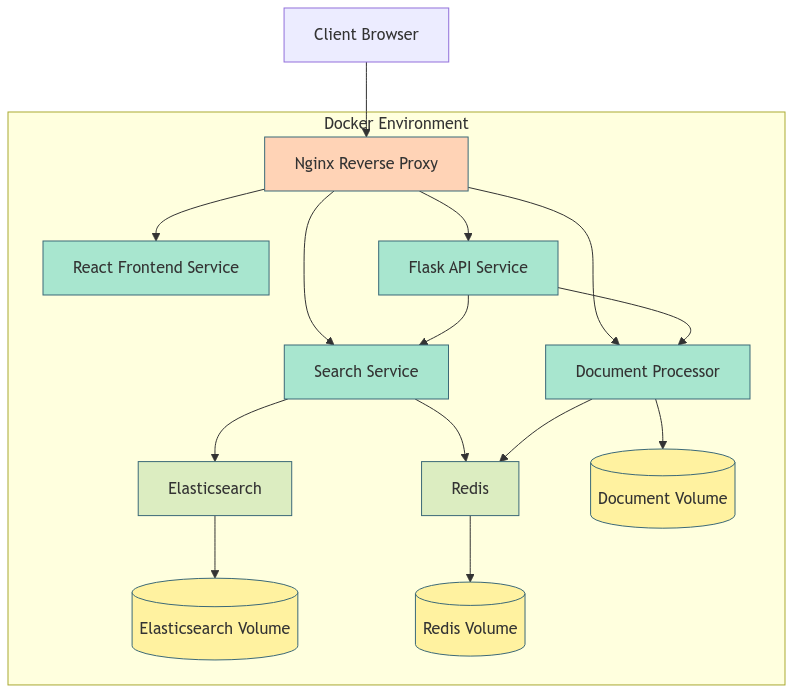
\includegraphics[width=0.95\textwidth,height=0.7\textheight,keepaspectratio]{systemarch.png}
    \end{column}
  \end{columns}
\end{frame}

\begin{frame}[fragile]{Docker Setup and Operations}
  \begin{columns}[T] % 'T' aligns columns at the top
    \begin{column}{0.48\textwidth} % Slightly reduced width for margin
      \begin{beamercolorbox}[shadow=true,rounded=true]{block title}
        \centering\textbf{Docker Compose Config}
      \end{beamercolorbox}
        \begin{verbatim}
services:
  nginx:
    image: nginx:alpine
    ports:
      - "4321:80"
  frontend:
    build: ./frontend
    expose:
      - "3000"
  api:
    build: ./api
    expose:
      - "8000"
  document-processor: (...)
  search: (...)
        \end{verbatim}
    \end{column}
    
    \hspace{0.5em} % Add horizontal space between columns
    
    \begin{column}{0.48\textwidth}
      \begin{beamercolorbox}[shadow=true,rounded=true]{block title}
        \centering\textbf{Common Commands}
      \end{beamercolorbox}

        \begin{verbatim}
# Build and start
docker-compose up --build

# Stop services
docker-compose down

# View logs
docker-compose logs -f

# Rebuild specific service
docker-compose build svc-name

# Show running containers
docker-compose ps
        \end{verbatim}
    \end{column}
  \end{columns}
\end{frame}

\begin{frame}{Docker Benefits}
  \begin{columns}[T]
    \begin{column}{0.32\textwidth}
        \begin{beamercolorbox}[shadow=true,rounded=true]{block title}
        \centering 
        
\includegraphics[width=0.4\textwidth]{coding.png}\\[0.3em]
        For Development
      \end{beamercolorbox}
      \begin{itemize}
        \item \textbf{Consistent Environment} \\[-0.4em]
        {\tiny no "works on my machine"}
        \item \textbf{Isolated Deps} \\[-0.4em]
        {\tiny no version conflicts}
        \item \textbf{Rapid Dev Cycle} \\[-0.4em]
        {\tiny fast startup, easy rollbacks}
      \end{itemize}
    \end{column}
    
    \hspace{0.2em}
    
    \begin{column}{0.32\textwidth}
\begin{beamercolorbox}[shadow=true,rounded=true]{block title}
        \centering 
        
\includegraphics[width=0.4\textwidth]{performance.png}\\[0.3em]
        For Performance
      \end{beamercolorbox}
      \begin{itemize}
        \item \textbf{Resource Efficiency} \\[-0.4em]
        {\tiny lightweight architecture}
        \item \textbf{Scalability} \\[-0.4em]
        {\tiny horizontal scaling}
        \item \textbf{Maintenance} \\[-0.4em]
        {\tiny simple updates, min downtime}
      \end{itemize}
    \end{column}
    
    \hspace{0.2em}
    
    \begin{column}{0.32\textwidth}
\begin{beamercolorbox}[shadow=true,rounded=true]{block title}
        \centering 
        
\includegraphics[width=0.4\textwidth]{security.png}\\[0.3em]
        For Security
      \end{beamercolorbox}
      \begin{itemize}
        \item \textbf{Vulnerability Management} \\[-0.4em]
        {\tiny image scanning, regular updates}
        \item \textbf{Instance Isolation} \\[-0.4em]
        {\tiny for processes and networks}
        \item \textbf{Security Features} \\[-0.4em]
        {\tiny access \& resource limits}
      \end{itemize}
    \end{column}
  \end{columns}
\end{frame}
}

{
\setbeamercolor{frametitle}{bg=darkgreen}



}

{
\setbeamercolor{frametitle}{bg=darkmidnightblue}
\begin{frame}[fragile]{Project Implementation and System Features}
    % Use T (top baseline) alignment for columns themselves
    \begin{columns}[T]
        % Left column with text
        \begin{column}{0.48\textwidth}
            \begin{itemize}
                \item \textbf{Multi-stage builds}
                \begin{itemize}\small
                    \item Optimized image sizes
                    \item Reduced attack surface
                \end{itemize}

                \vspace{0.2cm}
                
                \item \textbf{Docker Compose}
                \begin{itemize}\small
                    \item Service orchestration
                    \item Environment configuration
                    \item Network management
                \end{itemize}

                \vspace{0.2cm}
                
                \item \textbf{Volume Management}
                \begin{itemize}\small
                    \item Persistent data storage
                    \item Efficient data sharing
                \end{itemize}
                
            \end{itemize}

            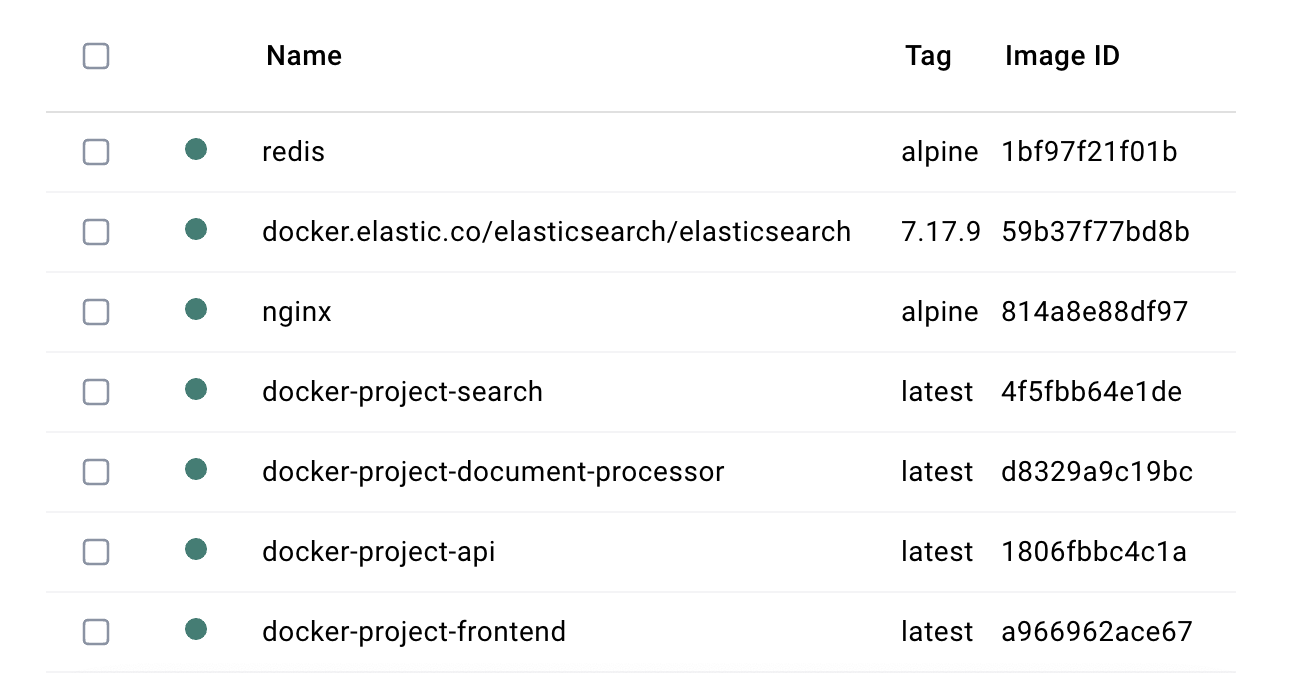
\includegraphics[width=0.95\textwidth,height=0.7\textheight,keepaspectratio]{docker_screenshot.png}
        \end{column}
        
        % Right column with image
        \begin{column}{0.48\textwidth}
            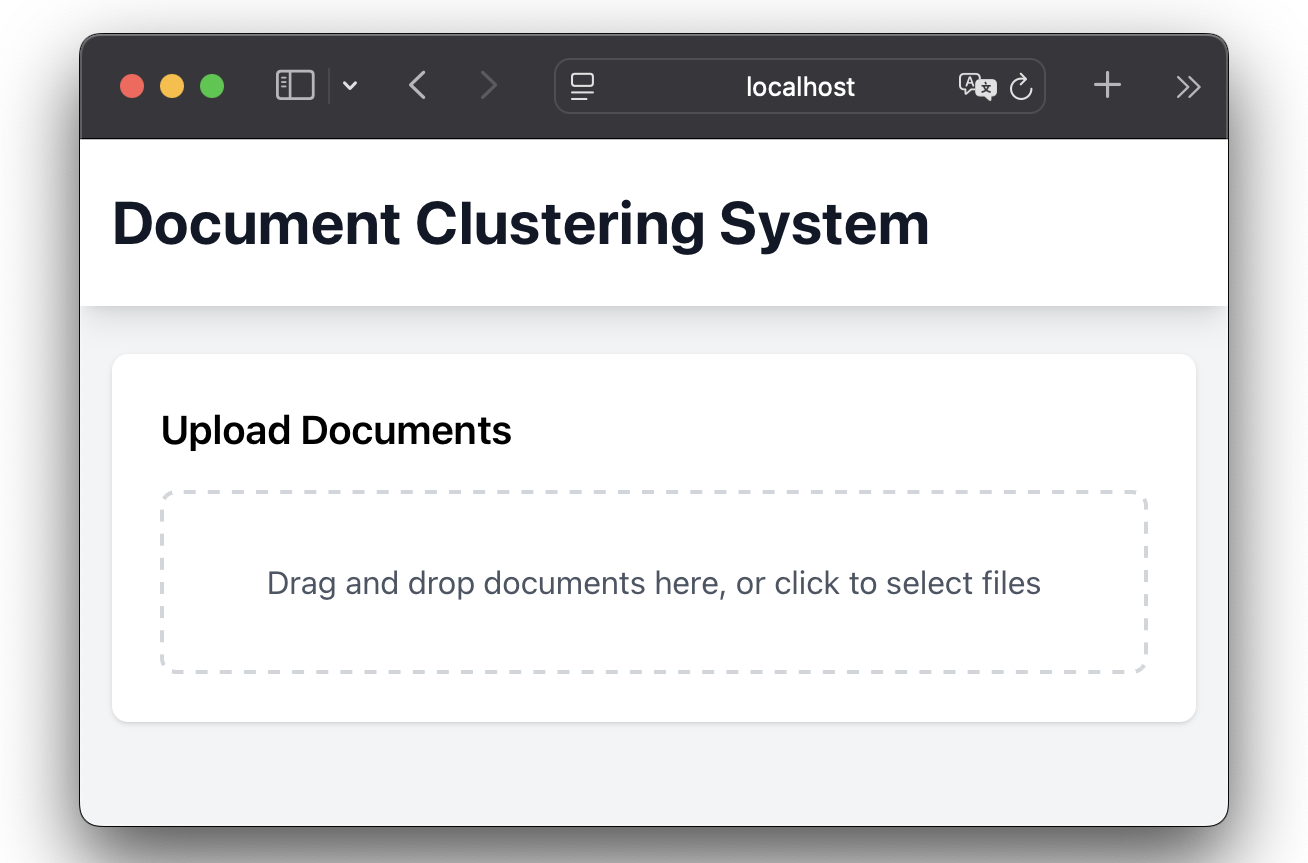
\includegraphics[width=0.9\textwidth,height=0.7\textheight,keepaspectratio]{app_screenshot.png}

            \begin{itemize}
                \item \textbf{Single Port Access}
                \begin{itemize}
                    \item All services through one port
                    \item Nginx reverse proxy
                    %\item Simplified deployment
                \end{itemize}
                \item \textbf{Monitoring}
                \begin{itemize}
                    \item Health checks
                    %\item Service discovery
                    \item Automated recovery
                \end{itemize}
                \item \textbf{Data Management}
                \begin{itemize}
                    \item Elasticsearch integration
                    \item Redis caching
                    \item Persistent storage
                \end{itemize}
            \end{itemize}
        \end{column}
    \end{columns}
\end{frame}
}

{
\setbeamercolor{frametitle}{bg=darkslateblue}
\begin{frame}{Managing Local and Production Environments}
    \textbf{Local Development: Docker Compose}
    \begin{itemize}
        \item Use \texttt{docker-compose.yml} for local setup.
        \item Benefits: ease of testing and configuration.
        \item Example commands:
        \begin{itemize}
            \item \texttt{docker-compose up --build}
            \item \texttt{docker-compose down}
            \item Add \texttt{docker-compose.override.yml} for environment-specific changes.
        \end{itemize}
    \end{itemize}
    \textbf{Production: Docker Swarm}
    \begin{itemize}
        \item Convert \texttt{docker-compose.yml} to Swarm using \texttt{docker stack deploy}.
        \item Enable high availability and service replication.
        \item Commands:
        \begin{itemize}
            \item \texttt{docker swarm init}
            \item \texttt{docker stack deploy -c docker-compose.yml <stack\_name>}
        \end{itemize}
    \end{itemize}
\end{frame}

\begin{frame}{Parallelizable Text Processing Tasks}
    \textbf{High-Load Document Processing Tasks}
    \begin{itemize}
        \item \textbf{OCR (Optical Character Recognition)}
        \begin{itemize}
            \item Divide documents into pages or segments.
            \item Use Tesseract with multiprocessing.
        \end{itemize}
        \item \textbf{Translations}
        \begin{itemize}
            \item Batch translations across multiple documents.
            \item Use APIs supporting parallel requests (e.g., Google Translate API, DeepL).
        \end{itemize}
        \item \textbf{Natural Language Processing (NLP)}
        \begin{itemize}
            \item Parallel topic modeling or sentiment analysis.
        \end{itemize}
        \item \textbf{Parallelization Frameworks}
        \begin{itemize}
            \item Celery with RabbitMQ or Redis.
            \item Python's \texttt{multiprocessing}, \texttt{joblib} for batch processing.
        \end{itemize}
    \end{itemize}
\end{frame}

\begin{frame}{Cloud Deployment with Blue-Green Strategy}
    \textbf{Cloud Platforms}
    \begin{itemize}
        \item \textbf{AWS:} Elastic Beanstalk, ECS/EKS for container orchestration.
        \item \textbf{Azure:} App Service, AKS for Kubernetes clusters.
        \item \textbf{DigitalOcean:} App Platform or Kubernetes droplets.
    \end{itemize}
    \textbf{Blue-Green Deployment}
    \begin{itemize}
        \item Keep two environments (blue = live, green = staging).
        \item Traffic shift via load balancer after validation.
        \item Benefits: zero-downtime upgrades and rollback safety.
    \end{itemize}
\end{frame}

\begin{frame}{Kubernetes with Docker Containers}
    \textbf{Why Kubernetes?}
    \begin{itemize}
        \item Advanced orchestration and scaling compared to Docker Swarm.
        \item Features: self-healing, automated rollouts.
    \end{itemize}
    \textbf{Key Components}
    \begin{itemize}
        \item Pods, Deployments, Services, ConfigMaps, and Ingress.
    \end{itemize}
    \textbf{Migration Process}
    \begin{itemize}
        \item Convert Docker Compose to Kubernetes manifests (\texttt{kubectl apply -f}).
        \item Use Helm charts for templating.
        \item Tools: Minikube for local testing, \texttt{kubectl} for CLI control.
    \end{itemize}
\end{frame}

\begin{frame}{Modern Docker-Based Approach vs Legacy System}
    \textbf{Legacy Approach}
    \begin{itemize}
        \item Monolithic deployments.
        \item Manual scaling and maintenance.
        \item Infrastructure tightly coupled.
    \end{itemize}
    \textbf{Docker-Based Approach}
    \begin{itemize}
        \item Microservices with independent scaling.
        \item Automated deployments and CI/CD.
        \item Isolated dependencies improve maintainability.
        \item Faster development cycles and simplified rollbacks.
    \end{itemize}
\end{frame}
}

\begin{frame}{Conclusion}
    \begin{center}
        \Large{Thank You}
        
        \vspace{0.5cm}
        \normalsize{Document Clustering System}\\
        Docker-based Microservices Architecture
        
        \vspace{0.5cm}
        Questions?
    \end{center}
\end{frame}


\end{document}